\documentclass[13pt]{article}

\usepackage{arxiv}

\usepackage{float}
\usepackage{graphicx}
\usepackage[utf8]{inputenc} % allow utf-8 input
\usepackage[T1]{fontenc}    % use 8-bit T1 fonts
\usepackage{hyperref}       % hyperlinks
\usepackage{url}            % simple URL typesetting
\usepackage{booktabs}       % professional-quality tables
\usepackage{amsfonts}       % blackboard math symbols
\usepackage{nicefrac}       % compact symbols for 1/2, etc.
\usepackage{microtype}      % microtypography
\usepackage{lipsum}

\usepackage{subcaption} 


\setlength{\parindent}{2em}
\setlength{\parskip}{1em}
\renewcommand{\baselinestretch}{1.2}

\title{An\'alisis y Caracterizaci\'on de instrumentos Musicales usando la transformada de fourier.}


\author{
  Ignacio Manuel Lebrero Rial \\%\thanks{Use footnote for providing further information about author (webpage, alternative address)---\emph{not} for acknowledging funding agencies.} \\
  Departamento de Computaci\'on\\
  Facultad de Ciencias Exactas y Naturales\\
  Unversidad de Buenos Aires \\
  \texttt{ignaciolebrero@gmail.com} \\
  751/13\\
  %% examples of more authors
   \And
 Nestor Dario Ocles Garcia \\
  Departamento de Computaci\'on\\
  Facultad de Ciencias Exactas y Naturales\\
  Unversidad de Buenos Aires \\
  \texttt{dario.ocles@gmail.com} \\
  633/15\\
  \And
  Matias Millassón\\
  Departamento de Computaci\'on\\
  Facultad de Ciencias Exactas y Naturales\\
  Unversidad de Buenos Aires \\
  \texttt{matiasmillasson@gmail.com} \\
  LU 131/13\\
  \And
   Joaq   Joaquín Romera\\

uín Romera\\
   Departamento de Computaci\'on\\
   Facultad de Ciencias Exactas y Naturales\\
   Unversidad de Buenos Aires \\
   \texttt{joakromera@gmail.com} \\
   183/16\\
}

\begin{document}
\maketitle

\begin{abstract}
   En este trabajo presentamos un análisis sobre audios de distintos instrumentos musicales e intentamos caracterizarlos definiendo una noci\'on de \textbf{Identidad Instrumental} para más adelante intentar clasificarlos automáticamente según la misma. Para empezar recopilamos grabaciones de un conjunto de instrumentos con el objetivo tratar de entender sus propiedades individuales y tener un set para hacer los experimentos. De este set surgieron algunas clasificaciones básicas basadas en el material de construcción del instrumento (metales, maderas) y su forma de ejecución (percusión, con arco, viento), a su vez la fuente del sonido (cuerda, viento) y su medio de excitación (arco, boquilla) sugirieron otras categorías. Estas, en parte, determinarían las cualidades especctrales del sonido de cada instrumento. En segundo lugar decidimos centrar nuestro análisis en una serie de descriptores según la representación del sonido en su dominio espectral, temporal, y según su contenido armónico. Utilizamos estos descriptores para entrenar un modelo que permita predecir a qué familia pertenece cada muestra. Según el grado de éxito de este modelo podremos especular si estos descriptores son relevantes para describir un instrumento musical o la familia a la cual pertenece, o si son relevantes para una determinada familia y no para otra. Finalmente intentamos lograr la separación de instrumentos en grabaciones que incluyan dos ejecutando notas diferentes al mismo tiempo, utilizando la decomposición de componentes y activaciones de su espectograma.
\end{abstract}


% keywords can be removed
\keywords{Transformada de Fourier \and Procesaminto de señales \and Instrumentos Musicales}

\clearpage

\section{Introduction}

\subsection{Problema General}

El análisis de instrumentos musicales es un problema clásico en el campo de la Recuperación de Información Musical (MIR, Music Information Retrieval) que a su vez representa un desafío de gran complejidad e interés en el ámbito. La clasificación de muestras de instrumentos según su timbre es un campo de investigación todavía abierto debido a esta complejidad. La música es una actividad artística esencial de la sociedad humana, diversos estudios ya trataron la clasificación de los instrumentos en jerarquías basadas en los materiales de fabricación de los instrumentos, así como en su fuente de sonido y su método de excitación, estos derivaron en las familias clásicas de instrumentos que se estudian desde hace casi dos siglos: instrumentos de cuerda (percutida, frotada con arco), de viento (maderas, metales), percusión, etc.

Gracias a los avances tecnológicos este análisis hoy se puede hacer sobre grabaciones digitales, estudiando la representación del sonido en distintos dominios facilitados por la transformada de Fourier (del tiempo, o de la frecuencia). Este acercamiento está basado directamente en el contenido que se puede extraer de las características del mismo audio del instrumento. Si la distinción hecha sobre materiales de construcción es una de alto nivel, podemos considerar este análisis como uno de bajo nivel. El problema que estaríamos intentando resolver entonces, es encontrar una correlación entre descriptores de bajo y alto nivel que permita identificar una muestra de un instrumento o por lo menos acercarlo a su familia según su descriptor de alto nivel.
        
\subsection{¿Qué hacemos en este trabajo?}

En la seccion 2 presentamos un breve análisis sobre audios de instrumentos aislados descargados del MIS dataset desarrollado en la Universidad de IOWA$^{[1]}$ para tratar de caracterizarlos, basándonos en una t\'ecnica ya conocida (Benetos, Kotti \& Kotropoulos, 2006)$^{[2]}$ armamos un modelo de ML para clasificar audios de acuerdo al instrumento que se toca, es útil aclarar que en esta parte solo usamos audios aislados tanto para entrenar como para predecir. Podemos decir que la caracterización de los instrumentos en esta parte queda dada por los features usados y el modelo entrenado.

Finalmente, en la secci\'on 3 experimentamos con la \textit{factorizacion no negativa de matrices} para descomponer un audio y tratar de analizar si es posible usar esto para aislar instrumentos. 

Las herramientas utilizadas en el trabajo fueron todas open source como Python, librosa \footnote{Librer\'ia open source sobre manipulaci\'on de sonido en Python https://librosa.github.io/librosa/ }, Jupyter Notebook, sklearn de Scipy.

Ademas, dentro de un repositorio es pueden encontrar los sources y datasets necesarios, en particular \href{https://github.com/ilebrero/Procesamiento-de-senales/tree/master/Non-negative-matrices/Caracterizacion%20de%20Instrumentos}{aqui} para la seccion 2 y \href{https://github.com/ilebrero/Procesamiento-de-senales/tree/master/Non-negative-matrices/Separacion_de_audios}{aqui} para la seccion 3. 

En el primero se pueden encontrar:
    
\begin{itemize}
    \item \textit{Src:} Contiene los archivos en python para correr el codigo.
    \item \textit{Audios:} Contiene los audios para generar el dataset de entrenamiento y de prueba.
    \item \textit{Notebooks:} Contiene los jupyter notebooks con los mismos experimentos que en este trabajo.
\end{itemize}

En el segundo simplemente la carpeta \textit{Notebooks} con la notebook y los audios necesarios para correr el experimento, notar que los archivos resultantes tambien se guardan en ese directorio.
\newpage
\section{Caracterizacion de un instrumento}

\subsection{Extracci\'on de Features}

Hoy se encuentran muchos descriptores de bajo nivel basados en el contenido espectral usados en este campo de investigación. Para intentar determinar el timbre de los instrumentos usamos cuatro: Zero Crossing Rate, Spectral Rolloff, Spectral Centroid, Spectral Flatness.

\begin{itemize}
    \item \textit{Zero-Crossing Rate:}  es la velocidad en la que el signo de una señal cambia entre positivo y negativo. Este feature suele dar buenos resultados para clasificar instrumentos percusivos.
        
    \item \textit{Spectral Rolloff:} es una medida de la forma de la señal. Se define para cada muestra como la frecuencia central para un bin del espectrograma de modo que al menos el 85\% de la energía del espectro en esta muestra está contenido en este bin y los de abajo. Esto se puede utilizar para, por ejemplo, aproximar la frecuencia máxima (o mínima) ya que mide la frecuencia donde se concentra un porcentaje de la distribución de magnitud.
        
    \item \textit{Audio Spectrum Centroid:} es una medida utilizada en el procesamiento digital de señales para caracterizar un espectro. Indica dónde está el centro de masa del mismo. Perceptualmente tiene una fuerte correlación con la impresión del brillo de un sonido.
        
    \item \textit{Audio Spectrum Flatness:} o el coeficiente de tonalidad, es otra medida del procesamiento de señales que sirve para caracterizar el espectro de un audio. Se mide típicamente en decibeles y provee una forma para cuantificar que tan tonal es un sonido, contrapuesto a que tan parecido al ruido es.
\end{itemize}

\subsection{Modelo}
\label{sec:modelo}


Parar el modelo usamos la \textit{factorización no negativa de matrices} (En adelante NMF). Esto es, dada una matriz no negativa $V$ de $n x m$ (m vectores de n dimenciones), es posible encontrar matrices no negativas $W$ y $H$ tal que
\begin{center}
    $V \approx WH$
\end{center}
donde $W$, de la forma $n x r$, contiene una base de vectores y $H$, de la forma $r x m$, contiene los pesos necesarios para aproximar la correspondiente columnas de $V$. En particular, $r$ se elige de manera arbitraria. Usualmente es bueno tomar un $r$ tal que $(n+m)r < nm$ de manera que la matriz resultante sea una versi\'on compresa de la original.
        
\subsection{Procesamiento de datos y experimentos}

\subsubsection{Dataset}

El set de sonidos utilizados incluyó platillos, violines, flautas, trombones, guitarra y trompetas, con apróximadamente 70 muestras de cada uno, todas del mismo largo y discretizadas usando 44.1 kHz de sampling rate. De estas tomamos un 10\% para test y el resto para entrenamiento. Por un lado podemos distinguir entre estos instrumentos aquellos que son percutidos -platillos y al ser cuerda percutida, la guitarra- de los que no, y los que son no-tonales -los platillos- de los tonales -el resto-.

A su vez las familias clásicas basadas en los descriptores de alto nivel los distinguen en cuerdas: guitarra, violín; vientos: trompeta, trombón, flauta; percusión: platillos. En la familia de los vientos también se distingue entre los metales (trombón y trompeta) y las maderas (flauta).

Estas muestras son distintas notas únicas de cada instrumento, o golpes si se trata de un platillo, con varias articulaciones dependiendo de las posibilidades de cada instrumento. Por lo que cada archivo de audio corresponde a un único instrumento, ejecutando una sola nota.

\subsubsection{Método de Clasificaci\'on según features}

Extrayendo los features previamente dichos, generamos un vector de features $v_j$ por cada audio y con eso armamos la matriz $V$ donde cada $v_j$ representa una columna de la misma. Además, al saber de qué instrumento es cada audio guardamos un vector $l$ con los labels de cada columna de $V$.

El entrenamiento del modelo consiste en aplicar NMF a $V$ para calcular $W$ y $H$. Luego calculamos la pseudo inversa $W^{-1}$.

Finalmente, para estimar un nuevo audio, generamos su vector de features $v_{test}$ y hacemos:

\begin{center}
    $h_{test} = W^{-1} v_{test}$
\end{center}

Solo nos queda matchear de alguna manera con los vectores $h$ que ya calculamos y estimar el label. Para esto usamos $KNN$ comparando $h_test$ contra los vectores columna de $H$ y consideramos los más cercanos a los que minimizan la \textit{distancia euclidea} entre ellos, esto es, los que minimizan la norma de la resta. Originalmente probamos maximizando \textit{Cosine Similarity}, pero esta medida no di\'o buenos resultados. 
    
\subsubsection{Evaluaci\'on}

Los parametros con los que experimentamos fueron por un lado las \textit{n componentes} sobre la factorizacion NMF, este ser\'ia el \textit{r} de la factorizacion (que tanto comprimimos los datos o que factores tenemos en cuenta). Por otro lado probamos con distintos valores de \textit{k} para los k vecinos mas cercanos. Finalmente maximizamos la performance en los valores \textbf{6} y \textbf{4} para \textbf{n\_components} y \textbf{k} correspondientemente. A continuacion mostramos los resultados obtenidos corriendo el modelo con estos parametros y comparando el uso de distintos features isolados para tratar de entender como estos impactan en la predicci\'on:

\begin{figure}[h!]
    \centering
    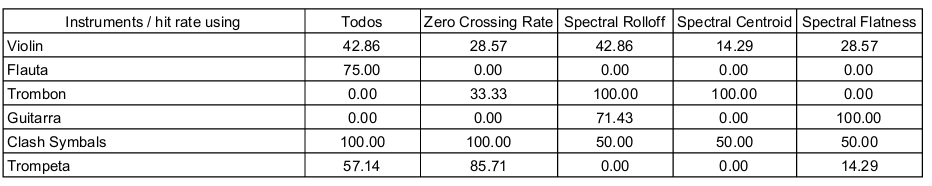
\includegraphics[scale=0.5]{Content/Figures/Comparacion_Features_Intrumentos.png}
    \caption{Resultados: Hit rate}
    \label{fig:resultados}
\end{figure}

\subsubsubsection{\textbf{Zero Crossing Rate}}

Era esperable que este descriptor de buenos resultados con instrumentos percusivos y en efecto los platillos fueron identificados correctamente en un 100\%.

\subsubsubsection{\textbf{Audio Spectral Roll-off}}

El descriptor de spectral roll-off arrojó buenos resultados para identificar las muestras de trombones y guitarras en menor medida.

\subsubsubsection{\textbf{Audio Spectrum Centroid}}

Consideramos que el 'brillo' de un sonido es una de las formas más sencillas de caracterizar y diferenciar sonidos, la formalización de esta característica corresponde a una indicación de la cantidad de energía en las frecuencias más altas de un sonido y es lo que podemos medir mediante el centroide espectral.

Llevado este análisis a los instrumentos estudiados encontramos un buen grado de precisión para el trombón. Sin embargo, el resultado no tiene una buena correlación con los descriptores de alto nivel dado que el trombón pertenece a la misma familia que la trompeta (vientos y metales) y es de un registro más grave, por lo que si obtuvimos buenos resultados con el trombón, hubieramos esperado obtener aún mejores resultados con la trompeta, ya que al ser de la misma familia y de un registro más agudo, debería haber mejorado su predicción con respecto al brillo.

\subsubsubsection{\textbf{Audio Spectral Flatness}}

Cuantificar qué tan tonal es un sonido no debería permitir distinguir instrumentos cuando son todos tonales, en nuestro set el único que se diferencia en esta dimensión son los platillos, que al ser inarmónicos deberían presentar diferenciarse facilmente de los demás.

Sin embargo, este desriptor no fue suficiente para lograr identificar esta distinción, el grado de precisión que arrojaron las muestras de platillos sugieren que este descriptor no alcanza para evidenciar esta hipótesis. En cuanto a la precisión que obtuvimos al predecir con los samples de guitarras, podemos suponer que la cualidad tonal de los mismos resultó más homogénea para este instrumento que para el resto.

\subsubsubsection{\textbf{Todos los descriptores combinados}}

Combinando todos los descriptores obtuvimos buenos resultados para identificar platillos en nuestro set de muestras, esta identificación mejoró a la obtenida por los descriptores separados (a excepción de Zero Crossing Rate, que dio igual). Esta combinación también mejoró la identificación de flautas, con el hecho notable de que por separado ningún descriptor había mostrado buena precisión. También mejoró la identificación de violines, aunque la precisión sigue siendo baja (por debajo del 50\%).

En el resto de los instrumentos vimos caer la precisión entre combinar los descriptores y utilizarlos por separado. No podemos afirmar que estos descriptores sean igual de determinantes para cada instrumento, ni para cada familia de instrumento, tampoco que mientras más descriptores combinemos, mejores resultados obtengamos. Es posible que los descriptores elegidos sean relevantes para los instrumentos percusivos inarmónicos (como los platillos) y no para los armónicos o melódicos (el resto). Una continuación de este trabajo debería constatar estos resultados con otros instrumentos percusivos e incluir descriptores nuevos para probar si pueden distinguir aquellos que producen sonidos armónicos entre sí.

Asi, podemos ver como queda la matriz de confusion resultante:

\begin{figure}[h!]
    \centering
    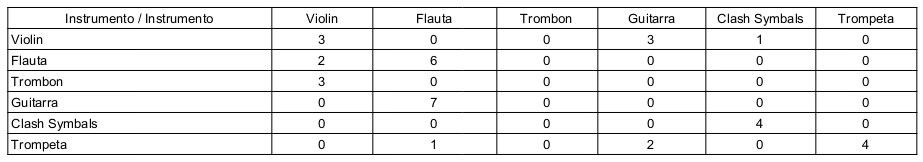
\includegraphics[scale=0.5]{Content/Figures/matriz-de-confusion.png}
    \caption{Matriz de Confusion entrenando con todos los features}
    \label{fig:my_label}
\end{figure}

Por lo que se muestra en la misma tiene bastante concentración en la diagonal para la flauta y clash cymbals mientras que para el resto de los instrumentos no hubo un gran desempeño. En particular todos los sonidos provenientes de las guitarras los clasificó como flautas pero se debe a que no analizamos tantos features. Con respecto a los violines su performance fue bastante buena ya que la gran mayoría de los sonidos los clasificó como violín o guitarra. Es decir las confusiones fueron sobre instrumentos de cuerda.
\newpage
% Esta parte se enfoca en la factorizacion de matriz no negativa y como dividimos los audios mergeados a mano
\section{Aislando Instrumentos}

Analizamos la posibilidad de separar audios de distintos instrumentos por medio de la factorizaci\'on NMF. Como se vio antes esta factorizaci\'on nos descompone el sonido en una matriz tiene una base de vectores y en otra matriz de activaci\'on de michos vectores. Realizamos dos experimentos, uno combinando una guitarra con una flauta y luego otro combinando una trompeta con un violín. Notar que en ambos casos mezclamos una instrumento de viento con uno de cuerda.

\subsection{Modelo}

El modelo es similar el propuesto en la secci\'on anterior \ref{sec:modelo} . Utilizamos la factorizaci\'on NMF y luego reconstruimos el sonido con dicha factorizaci\'on.
 
\subsection{Experimentaci\'on}

\subsubsection{Guitarra y flauta}

Experimentamos anulando algunos de estos vectores e intentamos reconstruir los audios originales por separado. Tomamos un audio de Guitarra (nota LA en 4ta octava) y un audio de Flauta (nota RE en 5ta octava), los mezclamos en un mismo audio superponiendo el sonido.

\begin{figure}[h!]
    \centering
    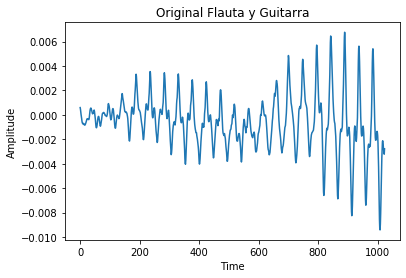
\includegraphics[height=60mm]{Content/Figures/separacion_original.png}
    \caption{Grafico del audio donde se mezclan Guitarra y Flauta}
\end{figure}

Luego separamos el audio en varios componentes usando la librer\'ia librosa para generar la matriz NMF. Con la matriz de factorizaci\'on fuimos anulando distintos vectores y reconstruyendo el audio con cada una de las nuevas matrices para luego quedarnos con aquellas matrices que tienen un mayor grado de correlaci\'on entre la matriz de factorizaci\'on de los audios por separado.
\\
\\
Con las nuevas matrices que tienen algunos vectores anulados pero que guardan mayor correlaci\'on con los sonidos originales reconstru\'imos el audio y los volvimos a graficar.

\begin{figure}[h!]
    \begin{subfigure}{0.5\textwidth}
        \centering
        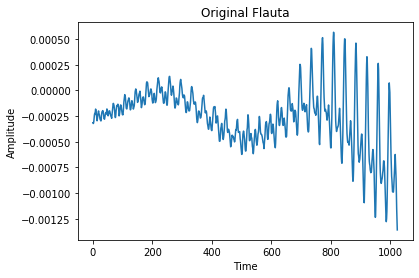
\includegraphics[height=60mm]{Content/Figures/separacion_audio1.png}
    \end{subfigure}
    \begin{subfigure}{0.5\textwidth}
        \centering
        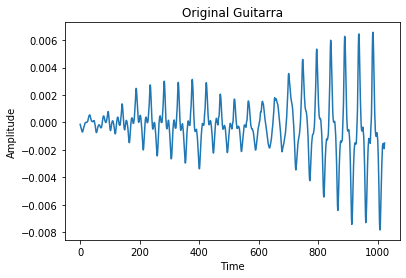
\includegraphics[height=60mm]{Content/Figures/separacion_audio2.png}
    \end{subfigure}
\end{figure}
\begin{figure}[h!]
    \begin{subfigure}{.5\textwidth}
        \centering
        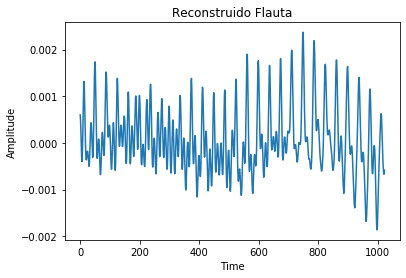
\includegraphics[height=60mm]{Content/Figures/separacion_reconstruccion_audio1.png}
    \end{subfigure}
    \begin{subfigure}{.5\textwidth}
        \centering
        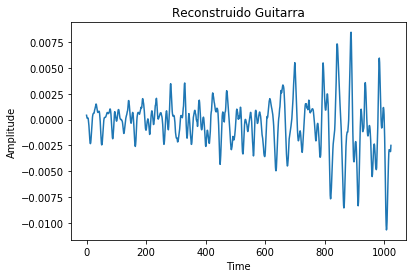
\includegraphics[height=60mm]{Content/Figures/separacion_reconstruccion_audio2.png}
    \end{subfigure}
\end{figure}

Como se puede observar, los audios reconstruidos mantienen un grado de similitud con los audios originales por separado. El sonido resultante de la reconstrucci\'on tambi\'en tienen un gran parecido con su audio original por separado a diferencia de otras tecnicas donde el audio reconstruido no guardaba mucha relaci\'on con el audio original.


Esta t\'ecnica podr\'ia ser util para la caracterizaci\'on de instrumentos como tambi\'en separaci\'on de audios. Con esta t\'ecnica no logramos separar audio en algunas de nuestras prueba indicando que esta t\'ecnica por si misma no es capaz de lograrlo. Sin embargo creemos que podr\'ia ser parte de t\'ecnicas m\'as avanzadas de caracterizaci\'on de sonido usando por ejemplo machine learning para detectar algunos aspectos del sonido.

\subsubsection{Violín y trompeta}
Al igual que en la sección anterior superpusimos los sonidos de dos instrumentos tocando una nota distinta. En este caso tomamos un violín y una trompeta. La nota correspondiente al sonido del violín es una D4, es decir octava prima de Re, en tanto la nota de la trompeta es una A4 lo que es lo mismo que una octava prima de La. La señal correspondiente a la mezcla se la puede ver en la siguiente figura:

\begin{figure}[h]
    \centering
    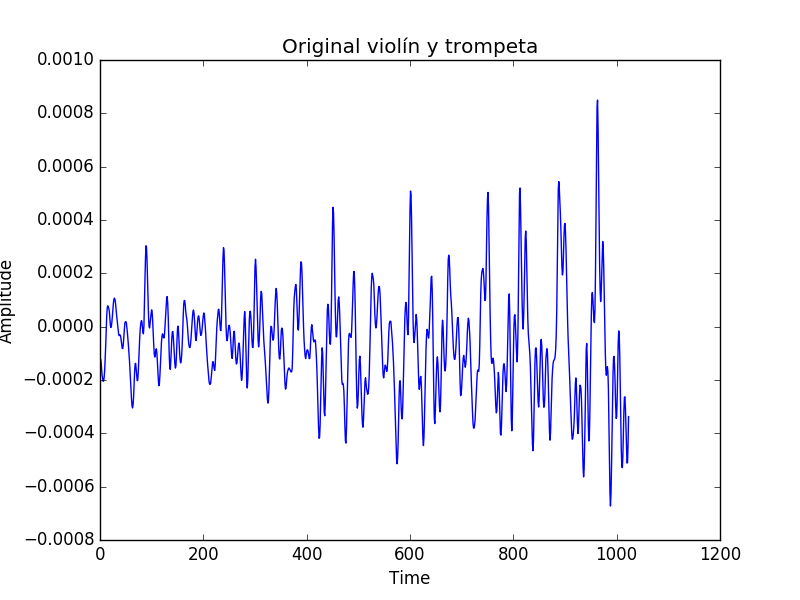
\includegraphics[height=60mm]{Content/Figures/orig_vio_trom.png}
    \caption{Grafico del audio donde se mezclan violín y trompeta}
\end{figure}

\newpage

Luego ejecutamos el script para separar la señal en las dos señales correspondientes a los instrumentos originales. Vale la pena aclarar que el script es exactamente el mismo que el que utilizamos para el experimento anterior.

\begin{figure}[h]
    \begin{subfigure}{0.5\textwidth}
        \centering
        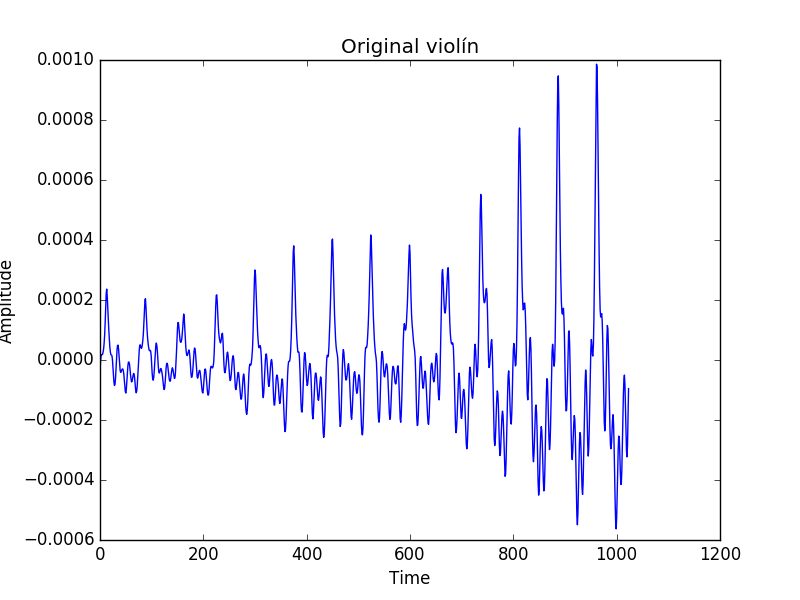
\includegraphics[height=60mm]{Content/Figures/orig_vio.png}
    \end{subfigure}
    \begin{subfigure}{0.5\textwidth}
        \centering
        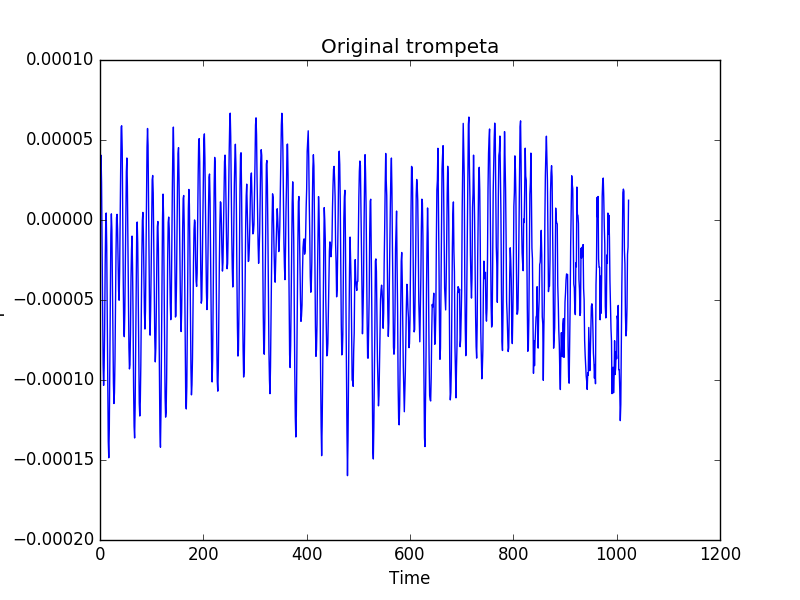
\includegraphics[height=60mm]{Content/Figures/orig_tromp.png}
    \end{subfigure}
\newline
    \begin{subfigure}{.5\textwidth}
        \centering
        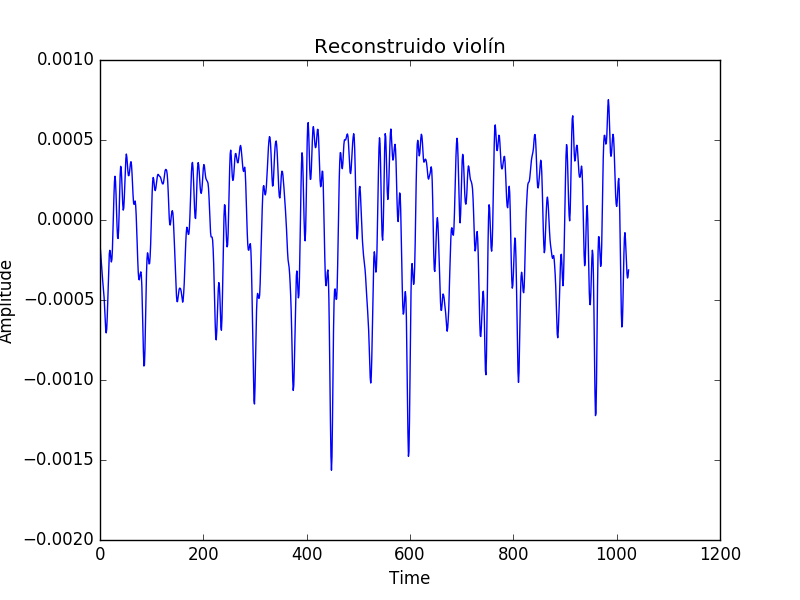
\includegraphics[height=60mm]{Content/Figures/recons_vio.png}
    \end{subfigure}
    \begin{subfigure}{.5\textwidth}
        \centering
        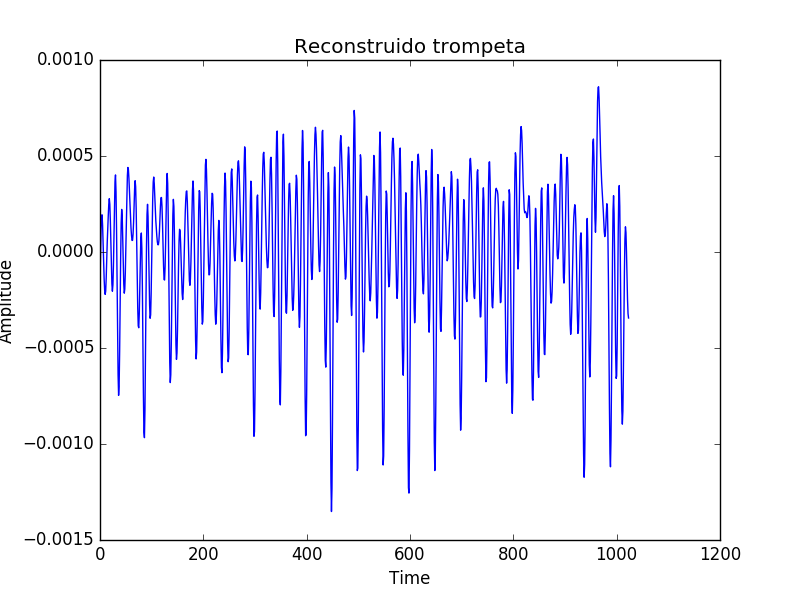
\includegraphics[height=60mm]{Content/Figures/recons_tromp.png}
    \end{subfigure}
\end{figure}

Como se puede apreciar en las figuras correspondientes a los audios originales la diferencia entre las señales es muy marcada pero en las versiones reconstruidas son similares. Además la trompeta se reconstruyó de manera satisfactoria mientras que el violín tiene bastantes diferencias. Por lo que podemos concluir que logró aislar correctamente la trompeta.

\newpage
\section{Conclusiones}

Podemos ver que caracterizar instrumentos y separar audio presesntan un desafio complejo para el cual existen una gamma de t\'ecnicas muy diversas para resolverlo. Ademas, la mayoria suele tener resultados parcialmente exitosos, de manera que resulta dificil resolver el problema de manera exacta y la manera de encararlo resulta ser estimando una soluci\'on relativamente buena.

En particular, la factorizaci\'on NMF nos fue muy util para descomponer el sonido en una cantidad arbitraria de componentes distintos. Esta factorizaci\'on es usada en distintas tecnicas de manipulaci\'on de audio pero usualmente resulta ser una pequena parte de un proceso mas grande para separar el audio.

Podemos ver que caracterizar instrumentos de manera "manual" en el sentido de intentar usar una tecnica particular resulta ser dificil para caracterizarlos, mas que nada debido a la cantidad de variables distintas a tener en cuenta sobre la senal, esto nos lleva a pensar que una solucion de ML puede llegar a ser la mas razonable para este tipo de problemas. Aun m\'as, nuestros resultados muestran como un modelo relativamente simple tiene una performance masomenos aceptable sobre un conjunto de datos, dejando abierta la pregunta de si se puede llegar a usar nuestro modelo como un modulo individual de un modelo mas grande.

Con respecto a la separaci\'on de audios, en nuestra experimentaci\'on logramos obtener casos donde dicha factorizaci\'on nos permitio separar alguna caracteristica del audio y relacionarla con el original, dando la idea de que este m\'etodo podr\'ia llegar a ser util como un modulo de un modelo mas grande, al igual que el modelo de ML.

%\lipsum[4] See Section \ref{sec:headings}.

%\subsection{Headings: second level}
%\lipsum[5]
%\begin{equation}
%\xi _{ij}(t)=P(x_{t}=i,x_{t+1}=j|y,v,w;\theta)= {\frac {\alpha _{i}(t)a^{w_t}_{ij}\beta _{j}(t+1)b^{v_{t+1}}_{j}(y_{t+1})}{\sum _{i=1}^{N} \sum _{j=1}^{N} \alpha _{i}(t)a^{w_t}_{ij}\beta _{j}(t+1)b^{v_{t+1}}_{j}(y_{t+1})}}
%\end{equation}

%\subsubsection{Headings: third level}
%\lipsum[6]

%\paragraph{Paragraph}
%\lipsum[7]
%
%\section{Examples of citations, figures, tables, references}
%\label{sec:others}
%\lipsum[8] \cite{kour2014real,kour2014fast} and see \cite{hadash2018estimate}.
%
%The documentation for \verb+natbib+ may be found at
%\begin{center}
  %\url{http://mirrors.ctan.org/macros/latex/contrib/natbib/natnotes.pdf}
%\end{center}
%Of note is the command \verb+\citet+, which produces citations
%appropriate for use in inline text.  For example,
%\begin{verbatim}
   %\citet{hasselmo} investigated\dots
%\end{verbatim}
%produces
%\begin{quote}
  %Hasselmo, et al.\ (1995) investigated\dots
%\end{quote}
%
%\begin{center}
  %\url{https://www.ctan.org/pkg/booktabs}
%\end{center}
%
%
%\subsection{Figures}
%\lipsum[10] 
%See Figure \ref{fig:fig1}. Here is how you add footnotes. \footnote{Sample of the first footnote.}
%\lipsum[11] 
%
%\begin{figure}
  %\centering
  %\fbox{\rule[-.5cm]{4cm}{4cm} \rule[-.5cm]{4cm}{0cm}}
  %\caption{Sample figure caption.}
  %\label{fig:fig1}
%\end{figure}
%
%\subsection{Tables}
%\lipsum[12]
%See awesome Table~\ref{tab:table}.
%
%\begin{table}
 %\caption{Sample table title}
  %\centering
  %\begin{tabular}{lll}
    %\toprule
    %\multicolumn{2}{c}{Part}                   \\
    %\cmidrule(r){1-2}
    %Name     & Description     & Size ($\mu$m) \\
    %\midrule
    %Dendrite & Input terminal  & $\sim$100     \\
    %Axon     & Output terminal & $\sim$10      \\
    %Soma     & Cell body       & up to $10^6$  \\
    %\bottomrule
  %\end{tabular}
  %\label{tab:table}
%\end{table}
%
%\subsection{Lists}
%\begin{itemize}
%\item Lorem ipsum dolor sit amet
%\item consectetur adipiscing elit. 
%\item Aliquam dignissim blandit est, in dictum tortor gravida eget. In ac rutrum magna.
%\end{itemize}
%
%
%\bibliographystyle{unsrt}  
%\bibliography{references}  %%% Remove comment to use the external .bib file (using bibtex).
%%%% and comment out the ``thebibliography'' section.
%
%
%%%% Comment out this section when you \bibliography{references} is enabled.
\begin{thebibliography}{1}
%

\bibitem{kour2014real}
University of Iowa Musical Instrument Sample Database,
\newblock http://theremin.music.uiowa.edu/index.html.

\bibitem{kour2014real}
Emmanouil Benetos, Margarita Kotti and Constantine Kotropoulos.
\newblock Musical instrument classification using non-negative matrix factorization algorithms.
\newblock In {\em Circuits and
Systems, 2006. ISCAS 2006. Proceedings. 2006 IEEE.
%\bibitem{kour2014fast}
%George Kour and Raid Saabne.
%\newblock Fast classification of handwritten on-line arabic characters.
%\newblock In {\em Soft Computing and Pattern Recognition (SoCPaR), 2014 6th
  %International Conference of}, pages 312--318. IEEE, 2014.
%
%\bibitem{hadash2018estimate}
%Guy Hadash, Einat Kermany, Boaz Carmeli, Ofer Lavi, George Kour, and Alon
  %Jacovi.
%\newblock Estimate and replace: A novel approach to integrating deep neural
  %networks with existing applications.
%\newblock {\em arXiv preprint arXiv:1804.09028}, 2018.
%
%\end{thebibliography}
%

\end{document}
